\documentclass[10pt]{article}
\usepackage{icmlko}

\icmlmeta{IP 파운데이션 월드모델}{144}{대조군을 고르는 손이 잡음보다 넓다}{노트 143의 이중차분에 귀무를 붙였더니 그 검정이 죽었고, 왜 죽었는지 파다가 현행 최고 정식화의 점수가 자기 입력에 귀착되지 않는 것을 찾았다}

\begin{document}

\twocolumn[
\icmlheader

\begin{abstract}
노트 143이 이중차분으로 나이 검정을 날카롭게 하고 ``평행추세 전제는 검정
안 했다''를 남겼다. 검정했다. 두 가지 귀무를 붙였다 --- 축을 임의로
처치·대조로 재배정하는 \textbf{위약}(평행추세를 직접 친다)과 나이를 섞는
\textbf{치환}(나이 효과가 없을 때). \textbf{먼저 내가 재현을 틀렸다} ---
후행 집합 안에서 나이를 갈랐는데 노트 142는 전체를 갈랐다. 전체로 다시
맞추니 모바일 $+$0.0947이 정확히 나온다. 그 위에서 답이 나왔다.
\textbf{모바일이 죽는다} --- 이중차분 $+$0.022, 위약 $p=0.617$, 나이 치환
$p=0.180$. 노트 142가 유일하게 걸고 등록부에 올린 그 도메인이다. 살아남는
것은 \textbf{도서}($p=0.003$/$0.017$)인데 원값이 $+$0.011로 아무도 안 걸었던
곳이다. 더 나쁜 것은 폭이다. 대조 집합을 손5 · 손5$+$검색 · 달력만 따위로
바꾸면 같은 도메인의 이중차분이 웹툰에서 $-$0.133$\sim$$+$0.045로 벌어지고,
그 폭이 귀무 표준편차의 \textbf{13.8배}다. 중앙 1.7배다. \textbf{대조군을
고르는 손이 잡음보다 넓으면 그것은 추정량이 아니다.} 그래서 채택 결정을
다시 냈고 --- 여기서 더 큰 것이 나왔다. 도메인마다 글·그림 축을 넣고 빼며
판을 견주는데, \textbf{팝업은 글·그림 축이 하나도 없는데 점수가 0.074
움직인다.} 입력이 한 비트도 안 바뀐 대상이다. 정식화 다섯을 같은 조작에
대 보니 능형 계열은 0.004$\sim$0.016이고 \textbf{현행 최고인 F8 부스팅만
0.074다.} 읽으려던 처치 효과는 0.003이었다. 열한째 가드 \textbf{귀착}을
붙인다 --- 남의 축 하나를 지우고 내 점수가 얼마나 움직이는지 실행마다
적는다. F8 0.077, 능형 0.025$\sim$0.029.
\end{abstract}
]

\begin{figure*}[t]
\centering
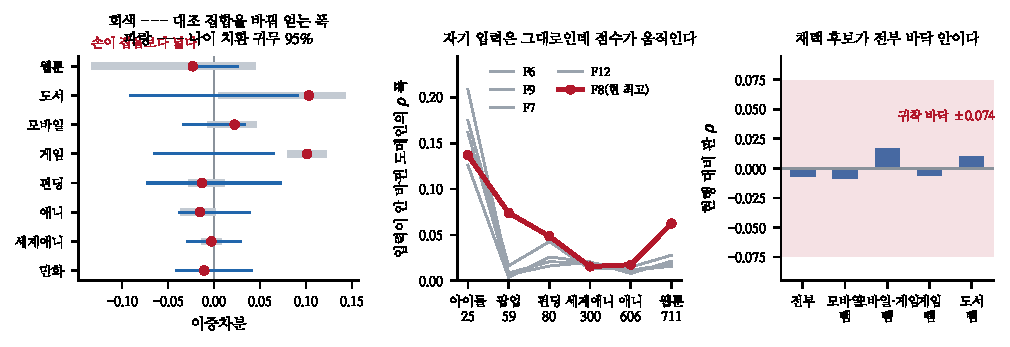
\includegraphics[width=\textwidth]{figs/attrib.pdf}
\caption{왼쪽 --- 대조 집합을 바꿔 얻는 폭(회색)이 귀무(파랑)보다 넓다.
가운데 --- 입력이 안 바뀐 도메인의 점수가 움직이는 폭. 오른쪽 --- 채택
후보가 전부 귀착 바닥 안이다.}
\end{figure*}

\section{먼저 재현을 틀렸다}

노트 142가 ``후행을 나이로 반 갈랐다''고 적었다. 그 문장을 후행 집합 안에서
가르는 것으로 읽고 다시 짰더니 모바일의 글·그림 나이차가 $+$0.095가 아니라
$-$0.004로 나왔다. 전체를 가르는 쪽으로 바꾸니 $+$0.0947이 소수 넷째까지
맞는다.

\claimx{\textbf{후행 안에서는 나이 효과가 아예 없다.} 모바일 전체
($n=2{,}000$, 중앙 2020.9)로 가르면 $+$0.095, 후행($n=441$, 중앙 2025.9)만
가르면 $-$0.004다. 나이 효과는 \emph{긴 밑변에서만} 보인다.}{이것 자체가
라벨 성숙 쪽 증거다. 설명문이 계속 갱신된다면 최근 1년 반 안에서도 갱신
차이가 있어야 한다. 다만 후행은 표본이 5분의 1이라 힘이 약하다.}

\section{귀무 둘}

\begin{table}[t]
\centering\tsize
\caption{이중차분(대조 전부)과 두 귀무의 $p$.}
\begin{tabular}{lrrrr}
\toprule
& 원값 & 이중차분 & 위약 & 나이치환 \\
\midrule
\textbf{도서} & $+$.011 & \textbf{$+$.103} & \textbf{.003} & \textbf{.017} \\
게임 & $+$.017 & $+$.101 & .086 & \textbf{.003} \\
\textbf{모바일} & \textbf{$+$.095} & $+$.022 & .617 & .180 \\
웹툰 & $+$.002 & $-$.023 & .528 & .070 \\
애니 & $-$.015 & $-$.015 & .570 & .463 \\
만화 & $-$.012 & $-$.011 & .501 & .627 \\
펀딩 & $-$.008 & $-$.013 & .620 & .740 \\
세계애니 & $+$.007 & $-$.003 & .889 & .860 \\
\bottomrule
\end{tabular}
\end{table}

위약은 축을 처치 20 · 대조 $k$로 \emph{임의} 재배정해 2{,}000번 다시
잰다. 평행추세가 성립하면 어떤 갈래든 이중차분이 0 근처여야 하므로, 이
분포가 곧 그 전제의 검정이다.

\claimx{\textbf{모바일이 죽는다.} 노트 142가 유일하게 걸고 등록부에 올린
도메인의 이중차분이 $+$0.022이고 두 귀무 다 통과 못 한다($p=0.617$ ·
$0.180$). 원값 $+$0.095의 4분의 3이 대조 축에도 똑같이 있었다.}{원값
$+$0.095 자체는 실재한다 --- 나이 치환 귀무에 대면 그것은 유의하다. 죽은
것은 ``그 나이차가 글·그림 축에 \emph{특유하다}''는 부분이다.}

\claimx{\textbf{살아남는 것은 아무도 안 걸었던 도서다}($p=0.003$/$0.017$).
그런데 도서의 원값은 $+$0.011로 0에 가깝다 --- 이중차분이 도서를 1위로
올리는 이유는 도서의 \emph{대조 축이} 음으로 갔기 때문이다.}{노트 143이
게임에 대해 똑같은 걱정을 적었다(``대조가 움직여서 생긴 것''). 그 걱정이
도서에서 더 크게 반복된다.}

\section{그리고 폭이 잡음보다 넓다}

대조 집합을 여섯 가지로 바꿔 봤다 --- 손 축 다섯만 · 손5$+$검색 ·
손5$+$달력 · 전부 · 검색만 · 달력만.

\begin{table}[t]
\centering\tsize
\caption{대조 집합에 따른 이중차분의 폭.}
\begin{tabular}{lrrrr}
\toprule
& 최소 & 최대 & 폭 & 폭/귀무sd \\
\midrule
\textbf{웹툰} & $-$.133 & $+$.045 & .179 & \textbf{13.8} \\
모바일 & $-$.008 & $+$.046 & .054 & 3.2 \\
도서 & $+$.005 & $+$.143 & .138 & 3.0 \\
애니 & $-$.037 & $+$.002 & .038 & 2.0 \\
세계애니 & $-$.014 & $+$.008 & .022 & 1.5 \\
게임 & $+$.080 & $+$.122 & .042 & 1.3 \\
펀딩 & $-$.027 & $+$.012 & .039 & 1.1 \\
만화 & $-$.013 & $-$.008 & .005 & 0.3 \\
\bottomrule
\end{tabular}
\end{table}

\claimx{\textbf{손이 잡음보다 넓다.} 대조군을 무엇으로 잡느냐가 웹툰에서
이중차분을 귀무 표준편차의 13.8배만큼 움직인다. 중앙이 1.7배다. 노트 143이
보고한 세 값(모바일 $+$.059 · 게임 $+$.082 · 웹툰 $-$.069)은 이 폭 안의
한 점이다.}{게임은 폭이 1.3배로 제일 좁고 나이 치환 $p=0.003$이다 ---
여덟 중 유일하게 값이 안정적이면서 유의하다. 다만 위약은 $p=0.086$이다.}

\section{채택을 다시 내려다 더 큰 것을 봤다}

\begin{table}[t]
\centering\tsize
\caption{F8 부스팅 · 검색$+$달력 위에 글·그림 축을 붙인다.}
\begin{tabular}{lrr}
\toprule
& 판 & 팝업 \\
\midrule
현행 (글·그림 없음) & $+$.3661 & $+$.4124 \\
$+$전부 & $+$.3589 & $+$.4351 \\
$+$모바일 뺌 & $+$.3572 & $+$.4375 \\
$+$모바일·게임 뺌 & \textbf{$+$.3826} & $+$.4764 \\
$+$게임 뺌 & $+$.3599 & $+$.4973 \\
$+$도서 뺌 & $+$.3762 & \textbf{$+$.5092} \\
\bottomrule
\end{tabular}
\end{table}

\textbf{팝업에는 글·그림 축이 하나도 없다.} 후보 축은 설명문과 표지에서
나오고 팝업 레코드에는 그 둘이 없다 --- 표에 든 여섯 판에서 팝업의 열은
전부 같다. 그런데 팝업 점수가 $+$0.4124에서 $+$0.5092까지 움직인다.

\claimx{\textbf{입력이 한 비트도 안 바뀐 대상의 점수가 0.097 움직인다.}
F8은 결정적이다(같은 자료 두 번 → 소수 다섯째까지 동일). 그러니 이것은
씨앗 잡음이 아니라 \emph{풀이 바뀌어서} 생긴 전파다.}{풀링 모형의 점수가
풀에 따라 변하는 것 자체는 정상이다. 문제는 크기다 --- 이 표에서 읽으려던
처치 효과가 0.003$\sim$0.017이다.}

\begin{table}[t]
\centering\tsize
\caption{입력이 안 바뀐 도메인의 $\rho$가 움직이는 폭. 다섯 판.}
\begin{tabular}{lrrrrr}
\toprule
후행 $n$ & F6 & F9 & F7 & F12 & \textbf{F8} \\
\midrule
아이돌 25 & .126 & .162 & .175 & .209 & .137 \\
\textbf{팝업 59} & .004 & .007 & .016 & .008 & \textbf{.074} \\
펀딩 80 & .026 & .016 & .043 & .021 & \textbf{.049} \\
세계애니 300 & .021 & .020 & .013 & .019 & .016 \\
애니 606 & .008 & .011 & .015 & .012 & .018 \\
웹툰 711 & .021 & .016 & .028 & .018 & \textbf{.062} \\
\midrule
중앙(아이돌 뺌) & .021 & .016 & .016 & .019 & \textbf{.049} \\
\bottomrule
\end{tabular}
\end{table}

\claimx{\textbf{현행 최고만 유독 크다.} 같은 도메인 · 같은 조작 · 같은
표본에서 F8이 팝업을 0.074 움직이는 동안 능형 계열은 0.004$\sim$0.016이다.
표본 크기 탓이 아니다 --- 제일 큰 웹툰($n=711$)에서도 F8 .062 대 F6
.021이다.}{아이돌($n=25$)은 모든 정식화에서 0.13$\sim$0.21 움직인다. 작은
표본은 무엇을 쓰든 안 흔들리게 못 한다.}

\section{가드 열한째 --- 귀착}

\claimx{\textbf{분해능이 ``표본이 작아 못 보는 차이''라면 귀착은 ``풀이
흔들려 못 돌리는 차이''다.} 대상이 아닌 도메인의 축을 임의로 하나 지우고
대상 점수가 얼마나 움직이는지 적는다. F8 0.077 · F6 0.029 · F9 0.025 ---
글·그림 축 스무 개를 통째로 넣고 빼는 조작과 다른 방식인데 같은 순서가
나온다.}{판정이 아니라 기록이다. 풀링 모형에서 이 값을 0으로 만들 수는
없다 --- 만들면 풀링이 아니다.}

\begin{table}[t]
\centering\tsize
\caption{누수 세 층과 한계 두 개.}
\begin{tabular}{lll}
\toprule
& 재는 것 & 노트 \\
\midrule
분해능 & 표본이 작아 못 보는 차이 & 135 \\
\textbf{귀착} & \textbf{풀이 흔들려 못 돌리는 차이} & \textbf{144} \\
\bottomrule
\end{tabular}
\end{table}

\section{그래서 무엇이 남나}

노트 142의 나이 검정과 노트 143의 이중차분은 둘 다 사후 탐지기로 쓸 수
없다. 등록부의 모바일 항목은 남긴다 --- 근거는 이제 자료가 아니라 ``앱스토어
목록은 갱신된다''는 상식 하나뿐이고, 노트 143에서 이미 그렇게 적어 뒀다.
글·그림 축은 채택하지 않는다. 방향이 틀려서가 아니라 \textbf{이 판에서
방향을 잴 수가 없어서다.}

\begin{table}[t]
\centering\tsize
\caption{남은 것.}
\begin{tabular}{ll}
\toprule
F8 & 왜 유독 전파가 큰가 --- 부스팅의 어떤 부분인가 \\
채택 & 도메인별 채택은 귀착 바닥 위에서만 가능하다 \\
게임 & 여덟 중 유일하게 안정적으로 걸린다 --- 자료가 없다 \\
\bottomrule
\end{tabular}
\end{table}

첫 줄이 다음 자리다. F8은 도메인 one-hot 을 자질로 넣은 부스팅이다. 트리가
분기를 고를 때 다른 도메인의 자질이 하나 사라지면 \emph{분기 구조 전체가}
다시 짜인다 --- 능형은 계수 하나가 조금 움직일 뿐이다. 그렇다면 전파의
크기는 트리 깊이와 자질 수에 달렸을 것이고, 그건 잴 수 있다.

\end{document}
